% Options for packages loaded elsewhere
\PassOptionsToPackage{unicode}{hyperref}
\PassOptionsToPackage{hyphens}{url}
%
\documentclass[
]{article}
\usepackage{amsmath,amssymb}
\usepackage{lmodern}
\usepackage{iftex}
\ifPDFTeX
  \usepackage[T1]{fontenc}
  \usepackage[utf8]{inputenc}
  \usepackage{textcomp} % provide euro and other symbols
\else % if luatex or xetex
  \usepackage{unicode-math}
  \defaultfontfeatures{Scale=MatchLowercase}
  \defaultfontfeatures[\rmfamily]{Ligatures=TeX,Scale=1}
\fi
% Use upquote if available, for straight quotes in verbatim environments
\IfFileExists{upquote.sty}{\usepackage{upquote}}{}
\IfFileExists{microtype.sty}{% use microtype if available
  \usepackage[]{microtype}
  \UseMicrotypeSet[protrusion]{basicmath} % disable protrusion for tt fonts
}{}
\makeatletter
\@ifundefined{KOMAClassName}{% if non-KOMA class
  \IfFileExists{parskip.sty}{%
    \usepackage{parskip}
  }{% else
    \setlength{\parindent}{0pt}
    \setlength{\parskip}{6pt plus 2pt minus 1pt}}
}{% if KOMA class
  \KOMAoptions{parskip=half}}
\makeatother
\usepackage{xcolor}
\IfFileExists{xurl.sty}{\usepackage{xurl}}{} % add URL line breaks if available
\IfFileExists{bookmark.sty}{\usepackage{bookmark}}{\usepackage{hyperref}}
\hypersetup{
  pdftitle={qPCR\_for\_faeces\_protocol},
  pdfauthor={Fay},
  hidelinks,
  pdfcreator={LaTeX via pandoc}}
\urlstyle{same} % disable monospaced font for URLs
\usepackage[margin=1in]{geometry}
\usepackage{color}
\usepackage{fancyvrb}
\newcommand{\VerbBar}{|}
\newcommand{\VERB}{\Verb[commandchars=\\\{\}]}
\DefineVerbatimEnvironment{Highlighting}{Verbatim}{commandchars=\\\{\}}
% Add ',fontsize=\small' for more characters per line
\usepackage{framed}
\definecolor{shadecolor}{RGB}{248,248,248}
\newenvironment{Shaded}{\begin{snugshade}}{\end{snugshade}}
\newcommand{\AlertTok}[1]{\textcolor[rgb]{0.94,0.16,0.16}{#1}}
\newcommand{\AnnotationTok}[1]{\textcolor[rgb]{0.56,0.35,0.01}{\textbf{\textit{#1}}}}
\newcommand{\AttributeTok}[1]{\textcolor[rgb]{0.77,0.63,0.00}{#1}}
\newcommand{\BaseNTok}[1]{\textcolor[rgb]{0.00,0.00,0.81}{#1}}
\newcommand{\BuiltInTok}[1]{#1}
\newcommand{\CharTok}[1]{\textcolor[rgb]{0.31,0.60,0.02}{#1}}
\newcommand{\CommentTok}[1]{\textcolor[rgb]{0.56,0.35,0.01}{\textit{#1}}}
\newcommand{\CommentVarTok}[1]{\textcolor[rgb]{0.56,0.35,0.01}{\textbf{\textit{#1}}}}
\newcommand{\ConstantTok}[1]{\textcolor[rgb]{0.00,0.00,0.00}{#1}}
\newcommand{\ControlFlowTok}[1]{\textcolor[rgb]{0.13,0.29,0.53}{\textbf{#1}}}
\newcommand{\DataTypeTok}[1]{\textcolor[rgb]{0.13,0.29,0.53}{#1}}
\newcommand{\DecValTok}[1]{\textcolor[rgb]{0.00,0.00,0.81}{#1}}
\newcommand{\DocumentationTok}[1]{\textcolor[rgb]{0.56,0.35,0.01}{\textbf{\textit{#1}}}}
\newcommand{\ErrorTok}[1]{\textcolor[rgb]{0.64,0.00,0.00}{\textbf{#1}}}
\newcommand{\ExtensionTok}[1]{#1}
\newcommand{\FloatTok}[1]{\textcolor[rgb]{0.00,0.00,0.81}{#1}}
\newcommand{\FunctionTok}[1]{\textcolor[rgb]{0.00,0.00,0.00}{#1}}
\newcommand{\ImportTok}[1]{#1}
\newcommand{\InformationTok}[1]{\textcolor[rgb]{0.56,0.35,0.01}{\textbf{\textit{#1}}}}
\newcommand{\KeywordTok}[1]{\textcolor[rgb]{0.13,0.29,0.53}{\textbf{#1}}}
\newcommand{\NormalTok}[1]{#1}
\newcommand{\OperatorTok}[1]{\textcolor[rgb]{0.81,0.36,0.00}{\textbf{#1}}}
\newcommand{\OtherTok}[1]{\textcolor[rgb]{0.56,0.35,0.01}{#1}}
\newcommand{\PreprocessorTok}[1]{\textcolor[rgb]{0.56,0.35,0.01}{\textit{#1}}}
\newcommand{\RegionMarkerTok}[1]{#1}
\newcommand{\SpecialCharTok}[1]{\textcolor[rgb]{0.00,0.00,0.00}{#1}}
\newcommand{\SpecialStringTok}[1]{\textcolor[rgb]{0.31,0.60,0.02}{#1}}
\newcommand{\StringTok}[1]{\textcolor[rgb]{0.31,0.60,0.02}{#1}}
\newcommand{\VariableTok}[1]{\textcolor[rgb]{0.00,0.00,0.00}{#1}}
\newcommand{\VerbatimStringTok}[1]{\textcolor[rgb]{0.31,0.60,0.02}{#1}}
\newcommand{\WarningTok}[1]{\textcolor[rgb]{0.56,0.35,0.01}{\textbf{\textit{#1}}}}
\usepackage{graphicx}
\makeatletter
\def\maxwidth{\ifdim\Gin@nat@width>\linewidth\linewidth\else\Gin@nat@width\fi}
\def\maxheight{\ifdim\Gin@nat@height>\textheight\textheight\else\Gin@nat@height\fi}
\makeatother
% Scale images if necessary, so that they will not overflow the page
% margins by default, and it is still possible to overwrite the defaults
% using explicit options in \includegraphics[width, height, ...]{}
\setkeys{Gin}{width=\maxwidth,height=\maxheight,keepaspectratio}
% Set default figure placement to htbp
\makeatletter
\def\fps@figure{htbp}
\makeatother
\setlength{\emergencystretch}{3em} % prevent overfull lines
\providecommand{\tightlist}{%
  \setlength{\itemsep}{0pt}\setlength{\parskip}{0pt}}
\setcounter{secnumdepth}{-\maxdimen} % remove section numbering
\ifLuaTeX
  \usepackage{selnolig}  % disable illegal ligatures
\fi

\title{qPCR\_for\_faeces\_protocol}
\author{Fay}
\date{23/01/2022}

\begin{document}
\maketitle

\hypertarget{quantitative-real-time-pcr-for-faecal-samples}{%
\subsection{Quantitative real-time PCR for faecal
samples}\label{quantitative-real-time-pcr-for-faecal-samples}}

\hypertarget{measuring-amount-of-dna-with-nanodrop}{%
\paragraph{Measuring amount of DNA with
NanoDrop}\label{measuring-amount-of-dna-with-nanodrop}}

\begin{itemize}
\tightlist
\item
  Switch on the PC next to nanodrop
\item
  Log in the program of NanoDrop
\item
  Add 1 µL of the solution, in which your DNA is diluted and blank
\item
  Write the sample name
\item
  Add 1 µL of your sample and measure
\item
  Save them on a usb stick
\end{itemize}

\hypertarget{standardizing-the-samples}{%
\paragraph{Standardizing the samples:}\label{standardizing-the-samples}}

\begin{itemize}
\tightlist
\item
  c1 = initial sample concentration
\item
  v1 = volume from initial stock
\item
  c2 = final concentration -- 50 ng/ µl
\item
  v2 = final volume -- 50 µl would be nice if possible
\end{itemize}

v1 = C2*v2 / c1 volume of water = v2 - v1

Easy way out: Add your results of the dna concentrations to an excel
table and calculate your results with these equation

\hypertarget{eimeria-specific-primers}{%
\paragraph{Eimeria specific primers:}\label{eimeria-specific-primers}}

Prepare the primers and make aliquots 1. Eim\_COI\_qX\_F
5'-TGTCTATTCACTTGGGCTATTGT-3' 2. Eim\_COI\_qX\_R 5'-GGA
TCACCGTTAAATGAGGCA-3'

\hypertarget{each-reaction-contains-20-uxb5l}{%
\subsubsection{Each reaction contains: (20
µL)}\label{each-reaction-contains-20-uxb5l}}

\begin{itemize}
\tightlist
\item
  1X iTaqTM Universal SYBRⓇ Green Supermix (Bio-Rad, USA)
\item
  400 nM forward and reverse primers
\item
  50 ng template gDNA
\end{itemize}

\hypertarget{steps-qpcr}{%
\paragraph{Steps qPCR:}\label{steps-qpcr}}

\begin{itemize}
\tightlist
\item
  Take out the samples /primers from the freezer and put them on ice
\item
  Prepare the layout of your plate
\item
  for every sample we have triplicates and a negative control per plate,
  which contains all the reagents without DNA (Water, SYBR and primers)
\item
  set up the plate and the run before you start on:
  \url{https://apps.thermofisher.com/}
\end{itemize}

\begin{figure}
\centering
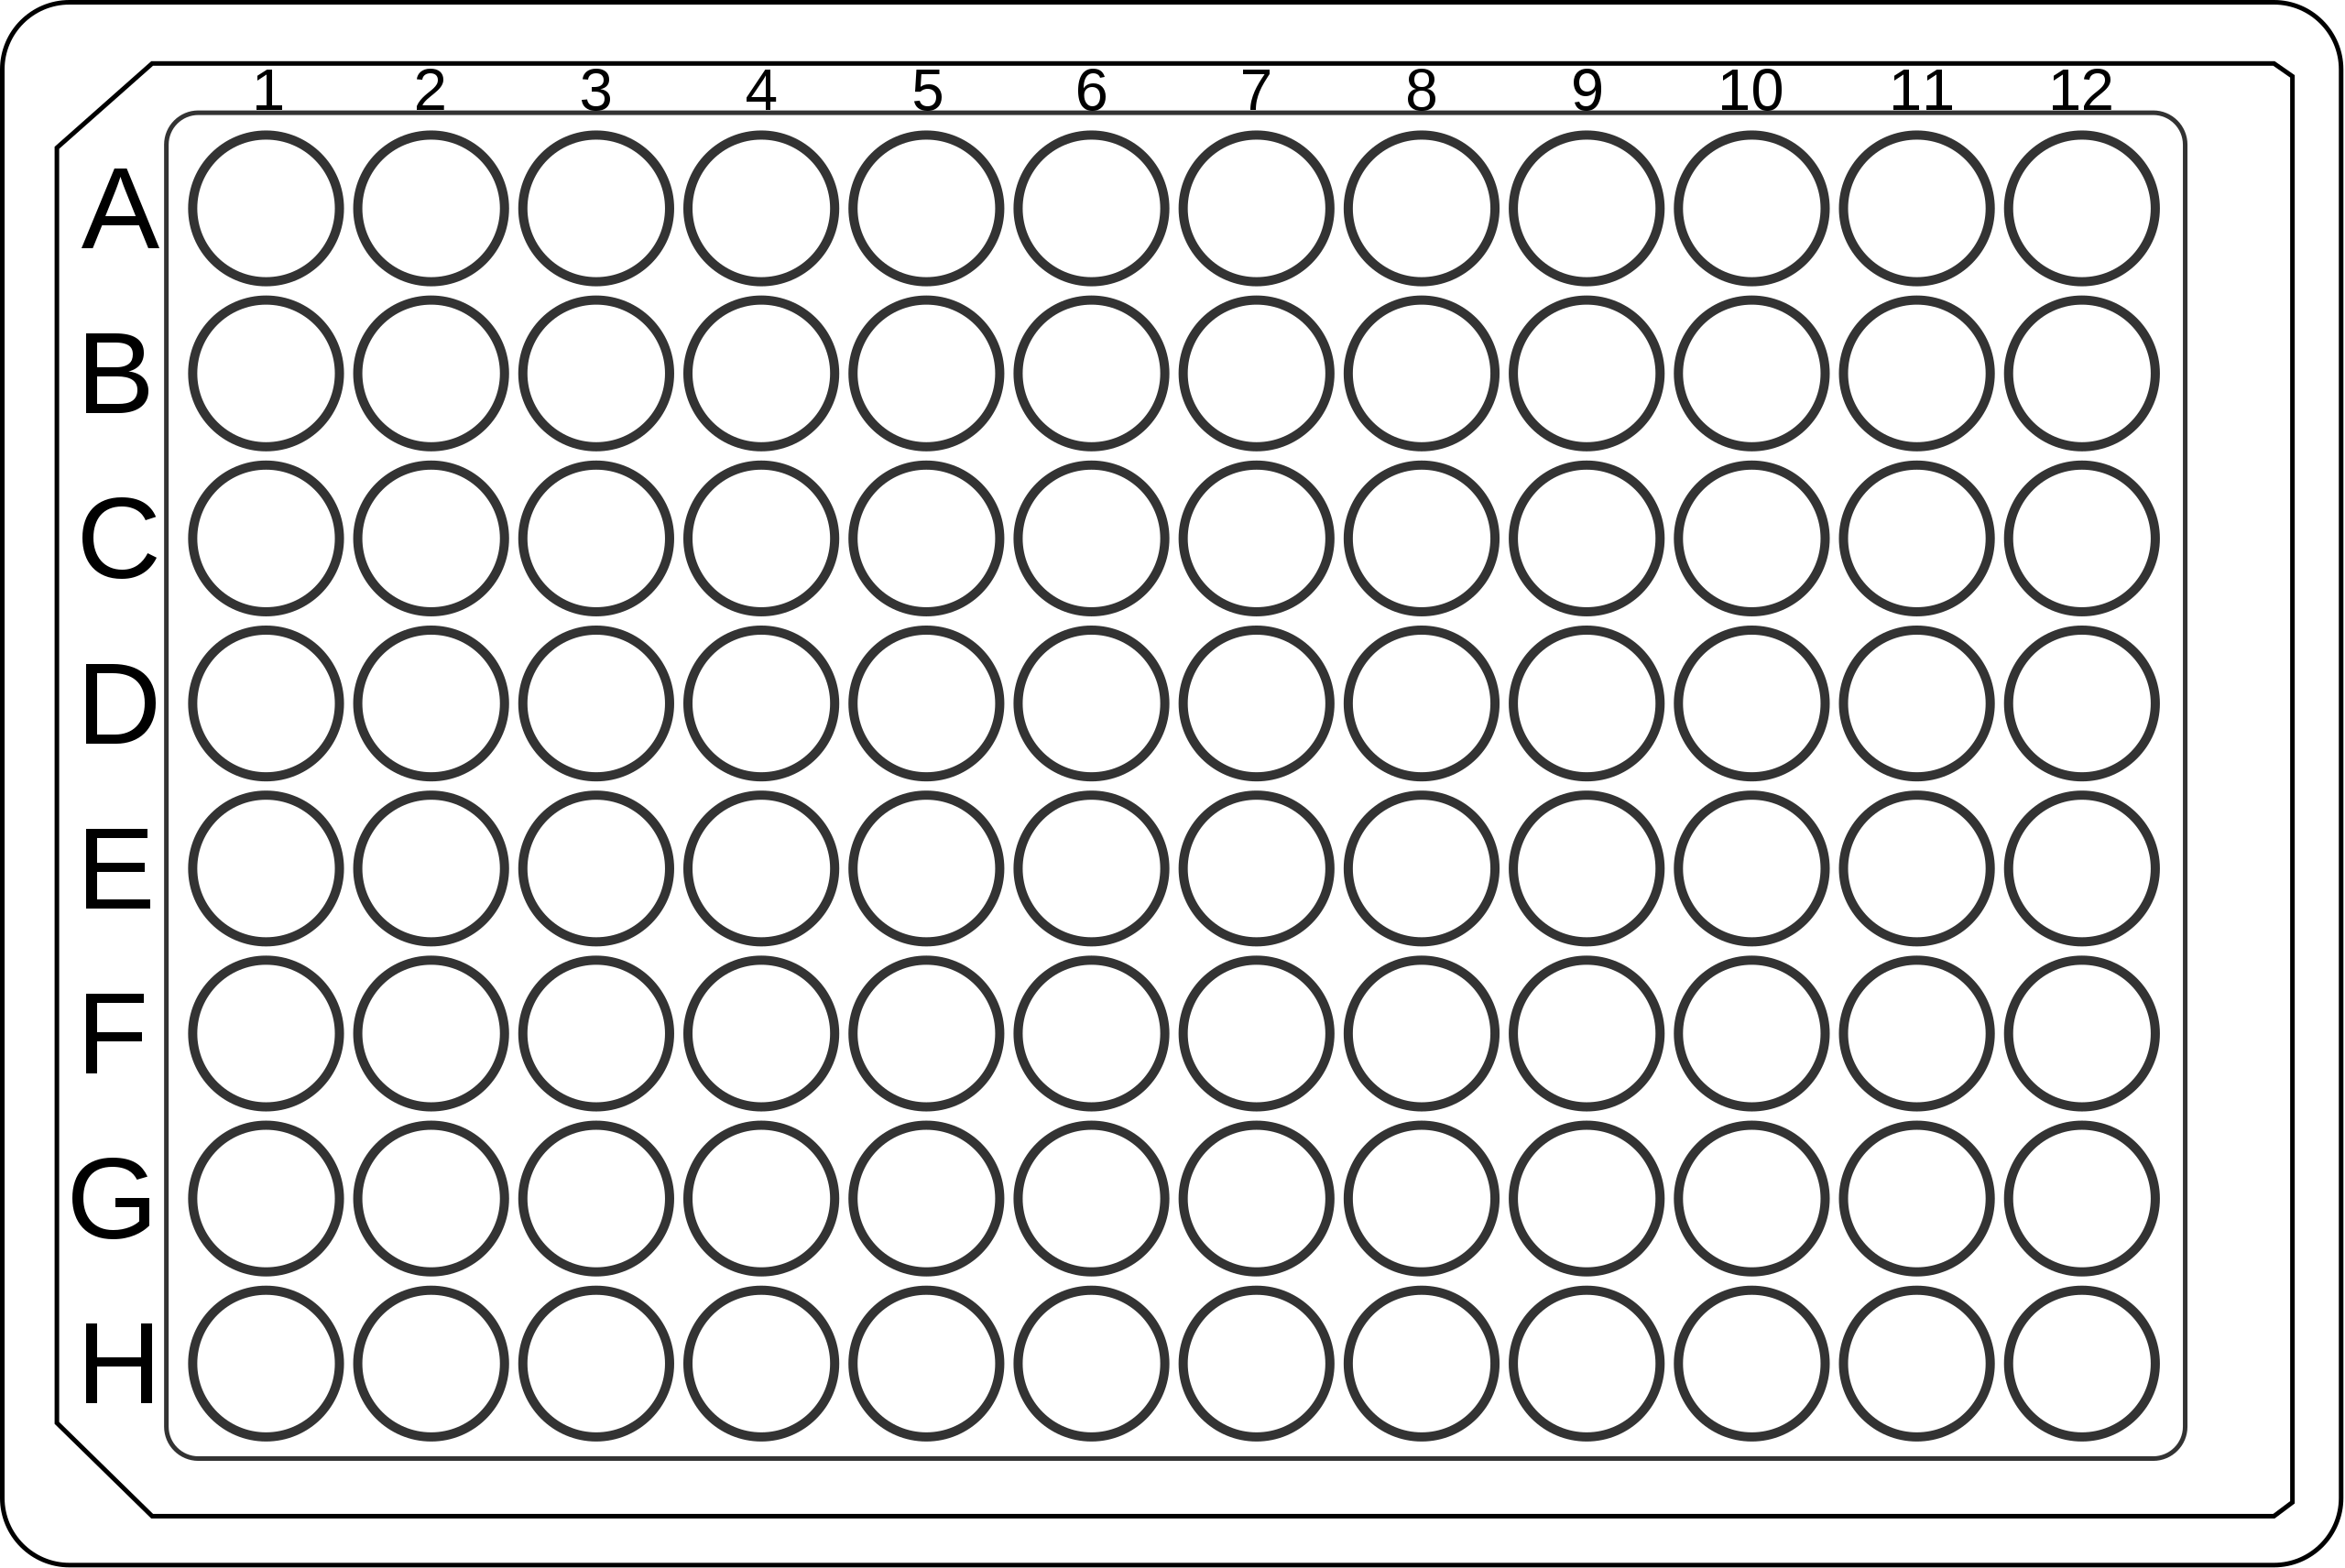
\includegraphics[width=3.125in,height=2.08333in]{96-Well_plate.png}
\caption{96 well layout}
\end{figure}

\hypertarget{recipe-for-one-reaction-20-uxb5l-per-well}{%
\paragraph{Recipe for one Reaction: (20 µL per
well)}\label{recipe-for-one-reaction-20-uxb5l-per-well}}

\begin{enumerate}
\def\labelenumi{\arabic{enumi}.}
\tightlist
\item
  SYBR: 10 µL
\item
  Forward primer: 0.8 µL
\item
  Reverse primer: 0.8 µL
\item
  H20: 7.4 µL
\item
  DNA: 1 µL of standardized 50 ng template gDNA
\end{enumerate}

\hypertarget{master-master-mix-prepare-in-eppendorf-tubes}{%
\paragraph{Master master mix: Prepare in Eppendorf
Tubes}\label{master-master-mix-prepare-in-eppendorf-tubes}}

n = sample + negative control number

\begin{Shaded}
\begin{Highlighting}[]
\NormalTok{n }\OtherTok{=} \DecValTok{17}
\NormalTok{STBR }\OtherTok{=} \DecValTok{10} \SpecialCharTok{*} \DecValTok{4} \SpecialCharTok{*}\NormalTok{ n}
\FunctionTok{cat}\NormalTok{(}\StringTok{"STBR = "}\NormalTok{, STBR,}\StringTok{"µL"}\NormalTok{)}
\end{Highlighting}
\end{Shaded}

\begin{verbatim}
## STBR =  680 µL
\end{verbatim}

\begin{Shaded}
\begin{Highlighting}[]
\NormalTok{FP }\OtherTok{=} \FloatTok{0.8} \SpecialCharTok{*} \DecValTok{4} \SpecialCharTok{*}\NormalTok{ n}
\FunctionTok{cat}\NormalTok{(}\StringTok{"Forward Primer = "}\NormalTok{, FP,}\StringTok{"µL"}\NormalTok{)}
\end{Highlighting}
\end{Shaded}

\begin{verbatim}
## Forward Primer =  54.4 µL
\end{verbatim}

\begin{Shaded}
\begin{Highlighting}[]
\NormalTok{RP }\OtherTok{=} \FloatTok{0.8} \SpecialCharTok{*} \DecValTok{4} \SpecialCharTok{*}\NormalTok{ n}
\FunctionTok{cat}\NormalTok{(}\StringTok{"Reverse Primer = "}\NormalTok{, RP,}\StringTok{"µL"}\NormalTok{)}
\end{Highlighting}
\end{Shaded}

\begin{verbatim}
## Reverse Primer =  54.4 µL
\end{verbatim}

\begin{Shaded}
\begin{Highlighting}[]
\NormalTok{H20 }\OtherTok{=} \FloatTok{7.4} \SpecialCharTok{*} \DecValTok{4} \SpecialCharTok{*}\NormalTok{ n}
\FunctionTok{cat}\NormalTok{(}\StringTok{"H20 = "}\NormalTok{, H20,}\StringTok{"µL"}\NormalTok{)}
\end{Highlighting}
\end{Shaded}

\begin{verbatim}
## H20 =  503.2 µL
\end{verbatim}

\hypertarget{master-mix-prepare-in-epis-or-strips}{%
\paragraph{Master mix: Prepare in epis or
strips}\label{master-mix-prepare-in-epis-or-strips}}

\begin{itemize}
\tightlist
\item
  76 µL MMM + 4 µL DNA template
\item
  Use a plate cooler with your plate
\item
  Finally pipette 20 µL in each well of the 96 plate for the reaction
\item
  File saved as:
  qPCR\_eimeria\_field\_faeces\_\_\_\_\_\_\_\_\_\_\_\_\_\_\_\_\_\_\_\_\_\_\_\_\_\_\_\_\_\_\_\_\_\_\_\_\_\_.eds
  in the thermofisher cloud
\end{itemize}

\hypertarget{pcr-machine}{%
\subsubsection{PCR machine:}\label{pcr-machine}}

\begin{itemize}
\tightlist
\item
  either in the ABI7300 Real-Time PCR system (Applied Biosystems, USA)
\item
  or in a MasterCycler® RealPlex2 (Eppendorf, Germany)
\item
  or in in the CFX96TM Touch System (Bio-Rad, USA)
\item
  QuantStudio 1 (Thermofisher)
\end{itemize}

\hypertarget{material-used}{%
\subsubsection{Material used:}\label{material-used}}

DNAs from mock samples, floated oocysts and faecal DNA derived from the
infection experiment

\hypertarget{cycling-conditions}{%
\subsubsection{Cycling conditions:}\label{cycling-conditions}}

Arrange the plate begore in Thermofischer.com Design Analysis new
--\textgreater{} set up plate --\textgreater{} comparative cd - SYBR

\begin{enumerate}
\def\labelenumi{\arabic{enumi}.}
\tightlist
\item
  initial denaturation at \textbf{95°C} for \textbf{2 min}
\item
  \textbf{40 cycles} of denaturation at \textbf{95°C} for \textbf{15 s}
\item
  annealing at \textbf{55 °C} for \textbf{15 s}
\item
  and extension at \textbf{68°} for \textbf{20 s}
\end{enumerate}

(with data collection at the end of each cycle)

\hypertarget{melting-curve-anaylsis}{%
\subsubsection{Melting curve anaylsis:}\label{melting-curve-anaylsis}}

Melting curve analysis was included to discard primer dimer formation
and non-specific amplification: after the last amplification cycle
temperature was increased from 65 °C to 95 °C with 0.5 °C increments at
3 s/step

\hypertarget{positioning-on-the-plate}{%
\subsubsection{Positioning on the
plate}\label{positioning-on-the-plate}}

Amplifications were performed by triplicate and each run included a
non-template control (NTC).

\hypertarget{analysis-and-interpretation}{%
\subsubsection{Analysis and
interpretation}\label{analysis-and-interpretation}}

Samples with all three replicates showing Tm (Melting curve temperature)
in the range 74.1 ± 1.78 °C (observed on positive controls, Additional
file 2: Figure S1) were labelled as ``qPCR positive'', samples with only
one or two of the triplicates showing peaks were designated as negative
samples.

For qPCR negative samples, genome copies per gram of faeces were set to
0. ict genome equivalents from Ct.

\end{document}
